\section*{Google PageRank}

Dalla sua nascita, Google ha impiegato brevissimo tempo per imporsi
come il pi\`u utilizzato motore di ricerca rispetto a tutti i
concorrenti. Il successo \`e dipeso dalla accuratezza delle risposte,
molto superiore a quelle di altri motori di ricerca.
Google infatti stila una propria classifica (\emph{ranking})
dell'importanza delle pagine web, per ordinare i risultati proposti;
molto spesso questa classifica \`e proprio quella desiderata l'utente.

L'algoritmo che ordina le pagine web per importanza \`e denominato
\emph{PageRank} ed \`e stato sviluppato da S.~Brin e L.~Page presso
la Stanford University \cite{Brin1998}.
Il principio su cui si basa \`e il seguente:
\begin{itemize}

    \item se una pagina web A ha un collegamento (\emph{link}) verso una
        pagina B, questo \`e interpretato come un voto di A in favore di B
        (cio\`e alza B in graduatoria);

    \item i votanti non sono tutti uguali: il voto di chi \`e alto in
        classifica (cio\`e ha ricevuto molti link) vale maggiormente di quello di chi \`e
        in basso.

\end{itemize}

\begin{figure}[htbp]
    \centering
    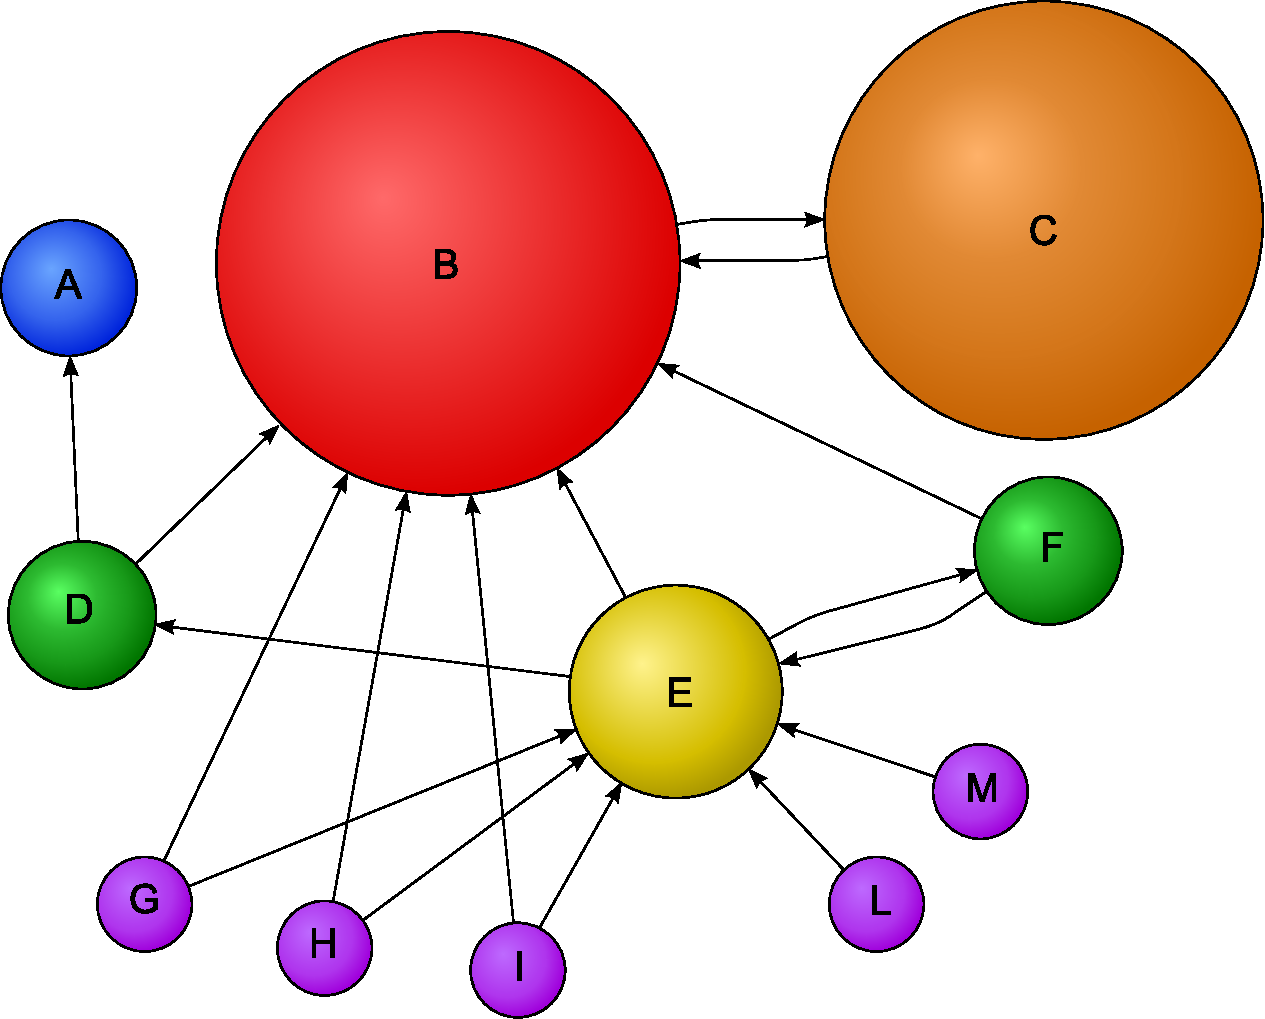
\includegraphics[width=0.6\textwidth]{./fig/PageRanks_Example_only_letters}
    \caption{Diagramma schematico del \emph{ranking}: ogni sfera rappresenta una pagina
            web, ogni freccia un link, la dimensione delle sfere \`e l'importanza
            attribuita alla pagina.}\label{fig:PR}
\end{figure}


Questo principio \`e descritto schematicamente in Fig.~\ref{fig:PR}.
La pagina B riceve molti link e quindi \`e considerata molto importante. La pagina
C \`e considerata pi\`u importante di E, anche se riceve meno link, perch\`e il voto di
B conta molto di pi\`u dei tanti ``piccoli'' voti che riceve E
(ad es. se il ``Washington Post'' o il ``New York Times'' pubblicassero un link al sito
web di ``Programmazione Avanzata per il Calcolo Scientifico'' questo varrebbe
molto di pi\`u dei link dai siti web personali di docente, esercitatore e studenti del corso!).

Dal punto di vista formale, si definisce il \emph{ranking} (importanza relativa) $r(p)$
della pagina $p$ come la somma di tutti i \emph{ranking} $r(q)$ di tutte le
pagine $q$ che puntano $p$:
\begin{align}
    \label{eq:rank}
    r(p)=\sum_{q \rightarrow p} \frac{r(q)}{\#q};
\end{align}
la somma \`e ponderata da $\#q$, numero di link presenti nella pagina $q$
(se una pagina $q$ ha un solo link verso $p$ \`e probabile che un lettore interessato lo segua,
viceversa se la pagina $q$ ha moltissimi link \`e poco probabile che il lettore scelga
proprio quello verso $p$).
\`E facile notare che si tratta di un problema in forma implicita: per conoscere il ranking di
$p$ si devono conoscere quelli delle altre pagine, che a loro volta si basano su quello di $p$.

Fortunatamente il problema \`e affrontabile in modo relativamente semplice, una volta scritto
in forma matriciale. Siano $\{p_1, p_2, \dots p_N\}$ tutte le pagine web censite e sia
$A \in \mathbb{R}^{N \times N}$ la matrice di connessione, il cui elemento $a_{i,j}$ \`e dato da:
\begin{align}
      \label{eq:harmonicp}
      a_{i,j}=
      \begin{cases}
        \dfrac{1}{\#p_j} &\qquad \mbox{se esiste un link da $p_j$ a $p_i$} \\[5mm]
        0 & \qquad \mbox{altrimenti.}
      \end{cases}
\end{align}

Si noti che gli $a_{i,j}$ possono essere intepretati come una distribuzione di probabilit\`a,
in particolare rappresentano la probabilit\`a che un persona che clicca a caso giunga alla
pagina $p_i$ a partire dalla pagina $p_j$. La matrice gode della propriet\`a:
\begin{align} \label{eq:sum1}
    \sum_{i=1}^{N} a_{i,j}=1.
\end{align}

Se il \emph{ranking} delle pagine web $p_i$ \`e rappresentato dal vettore colonn
\emph{PageRank} $\vv{r}=[r_1,r2, \dots r_n]^T$, allora l'equazione \eqref{eq:rank}
equivale al seguente problema:
\begin{align*}
    \vv{r}=A \vv{r}.
\end{align*}
Il \emph{PageRank} \`e quindi l'autovettore corrispondente all'autovalore 1 del problema
agli autovalori associato. Si pu\`o dimostrare che se i $\lambda_i$ sono gli autovalori
di $A$ allora $|\lambda_i| \leq 1$. Inoltre $\lambda_1=1$ ha molteplicit\`a
uno\footnote{Una condizione sufficiente \`e fornita dal teorema di Perron Frobenius,
che richiede una matrice corrispondente ad un grafo irriducibile. Un trucco per
soddisfare l'ipotesi potrebbe essere quello di attribuire un link ad ogni pagina
esistente alle pagine senza link.}.

Dato che il numero di pagine censite $N$ \`e dell'ordine di grandezza delle decine di
miliardi, il calcolo con un metodo diretto dell'autovettore \emph{PageRank} \`e
computazionalmente troppo oneroso, anche per chi dispone di risorse di calcolo eccezionali.
Si utilizza quindi un metodo iterativo, che restituisce una soluzione approssimata,
ad esempio ci si potrebbe basare sul metodo delle potenze. In questo caso particolare,
arrestare il numero di iterazioni al passo $k$ significa aver considerato solo le pagine
$p_j$ che distano da $p_i$ al pi\`u $k$ click\footnote{Per ragioni di semplicit\`a di
esposizione tralasciamo la possibilt\`a di introdurre un fattore di rilassamento
(\emph{damping fatctor}) \cite{Brin1998}, che comunque non modifica il principio base
dell'algoritmo.}.
